%%% Local Variables:
%%% mode: latex
%%% TeX-master: t
%%% End:

\documentclass[12pt]{article}
\usepackage[lmargin=1in,rmargin=1in,tmargin=1in,bmargin=1in]{geometry}

\usepackage{lmodern}			% Usa a fonte Latin Modern
\usepackage[T1]{fontenc}		% Selecao de codigos de fonte.
\usepackage[utf8]{inputenc}		% Codificacao do documento (conversão automática dos acentos)
\usepackage{indentfirst}		% Indenta o primeiro parágrafo de cada seção.
\usepackage{color}				% Controle das cores
\usepackage{graphicx}			% Inclusão de gráficos
\usepackage{microtype} 			% para melhorias de
% justificação
\usepackage{listings} %Inclusão de códigos de programação

\usepackage{enumitem} %enumerate com (a), (b), (c); (I), (II), etc

\usepackage[brazilian,hyperpageref]{backref}	 % Paginas com as citações na bibl
\usepackage[alf]{abntex2cite}	% Citações padrão ABNT\cos{}

% O tamanho do parágrafo é dado por:
\setlength{\parindent}{1.3cm}

% Controle do espaçamento entre um parágrafo e outro:
\setlength{\parskip}{0.2cm}  % tente também \onelineskip

\usepackage{./sty/design_ASC}

\setlength\parindent{0pt} %% Do not touch this

%% -----------------------------
%% TITLE
%% -----------------------------
\title{Problemas Capítulo \#7}

\vspace{4cm}


\author{Pedro G. Branquinho\\ %% Student name
  LOM3227 - Métodos da Física Computacional \\ %% Code and course name
  \textsc{Universidade de São Paulo}
}

\vspace{2cm}

\date{Abril, 2020 \\ (Os códigos estão nas pastas, nesse diretório, nomeadas por
problema. i.e., problema7.3 -> ./Cod\_73.)} %% Change "\today" by another date manually
%% -----------------------------
%% -----------------------------


%% %%%%%%%%%%%%%%%%%%%%%%%%%
\begin{document}
\setlength{\droptitle}{-5em}
%% %%%%%%%%%%%%%%%%%%%%%%%%%
\maketitle

% --------------------------
% Start here
% --------------------------

% %%%%%%%%%%%%%%%%%%%
\clearpage
\section*{Questão 7.3}
% %%%%%%%%%%%%%%%%%%%
{\bfseries
  \begin{equation}
    m \ddot x(t) + \epsilon \dot x(t) + k x(t) = F_e (t)
  \end{equation}
}

\subsection*{Respostas}

\subsubsection*{Q7.3(a),(b) gráfico $x(t)$ vs $t$ e $v(t)$ vs $t$}

\begin{figure}[!hbt]
  \begin{center}
    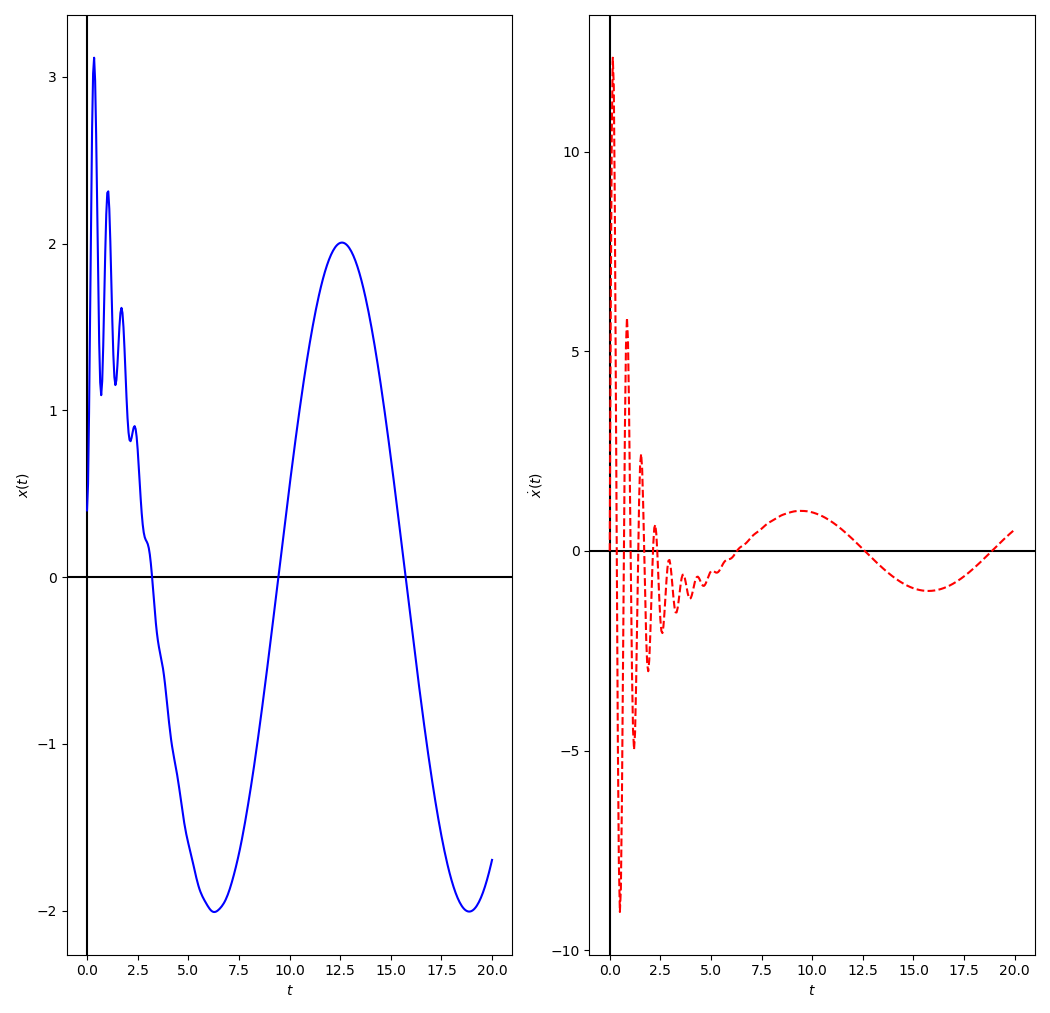
\includegraphics[scale=0.6]{./Cod_73/x(t)_v(t)}
  \end{center}
\end{figure}


\subsubsection*{Q7.3(c),(d) gráfico $E(t)$ vs $t$; $a(t)$ vs $t$}

\begin{figure}[!hbt]
  \begin{center}
    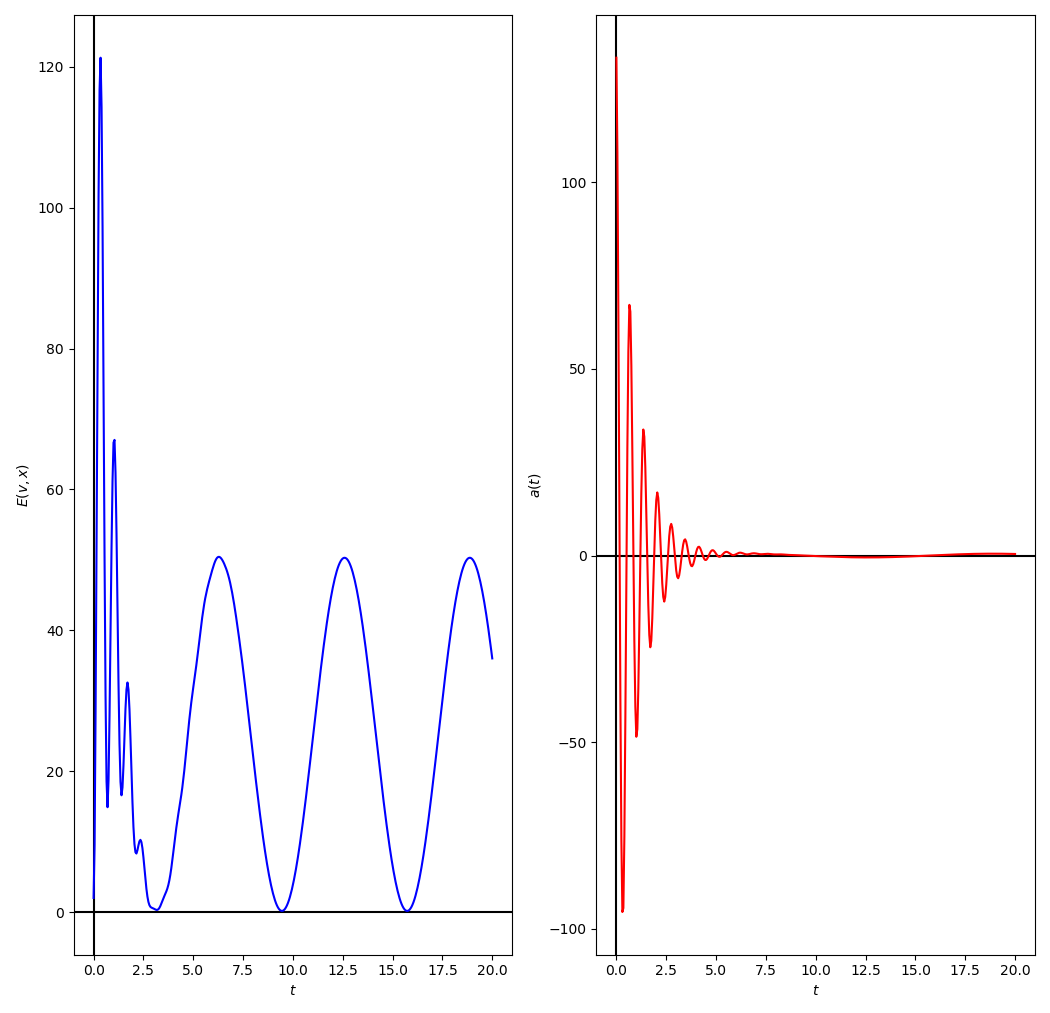
\includegraphics[scale=0.7]{./Cod_73/E(t)_a(t)}
  \end{center}
\end{figure}

\clearpage

\subsubsection*{Q7.3(e) gráfico $v(x)$ vs $x$}

\begin{figure}[!hbt]
  \begin{center}
    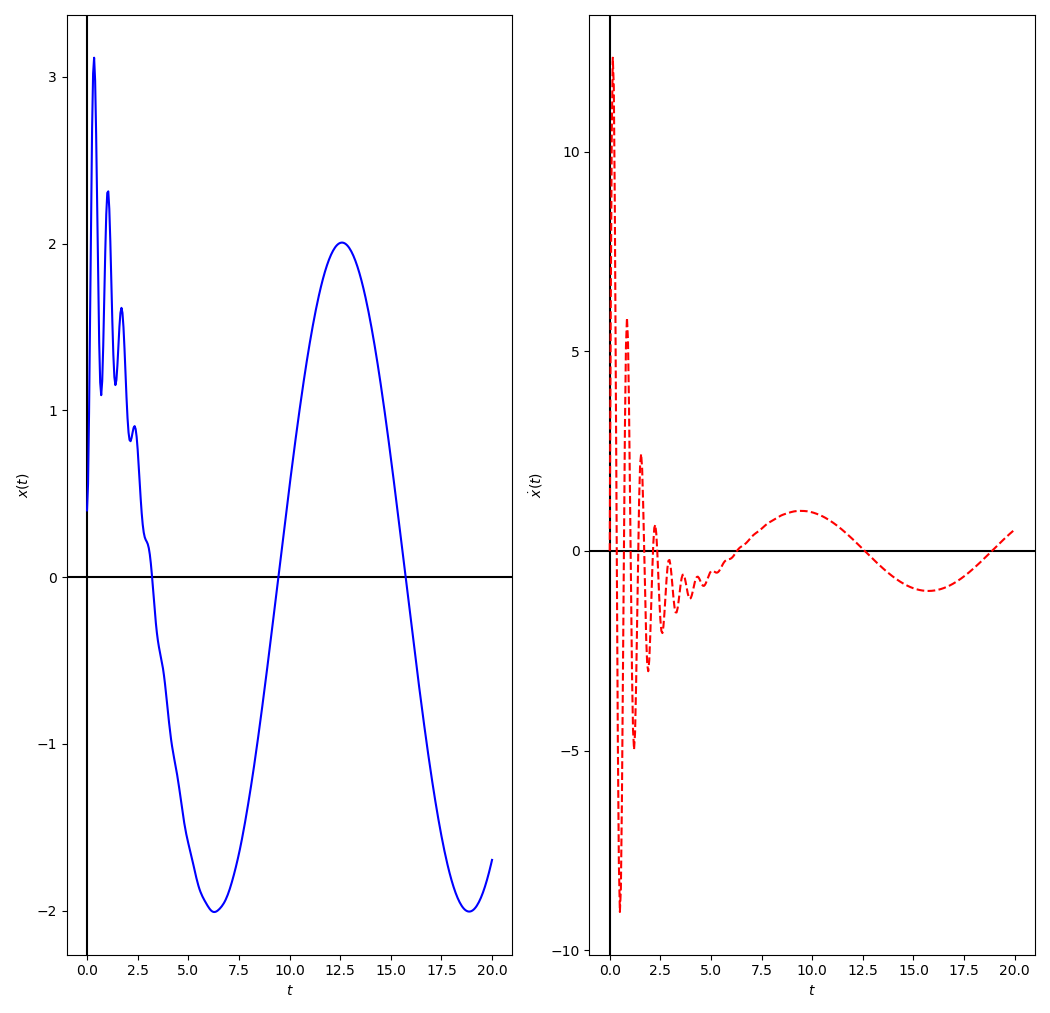
\includegraphics[scale=0.71]{./Cod_73/x(t)_v(t)}
  \end{center}
\end{figure}

% %%%%%%%%%%%%%%%%%%%
\section*{Questão 7.4}
% %%%%%%%%%%%%%%%%%%%
{\bfseries
  \begin{equation*}
      \ddot{x}(t) = -x - \epsilon (x^2 -1) \dot{x} \\
  \end{equation*}
}

\subsubsection*{Q7.4(a) gráfico $x(t)$ vs $t$}

\begin{figure}[!hbt]
  \begin{center}
    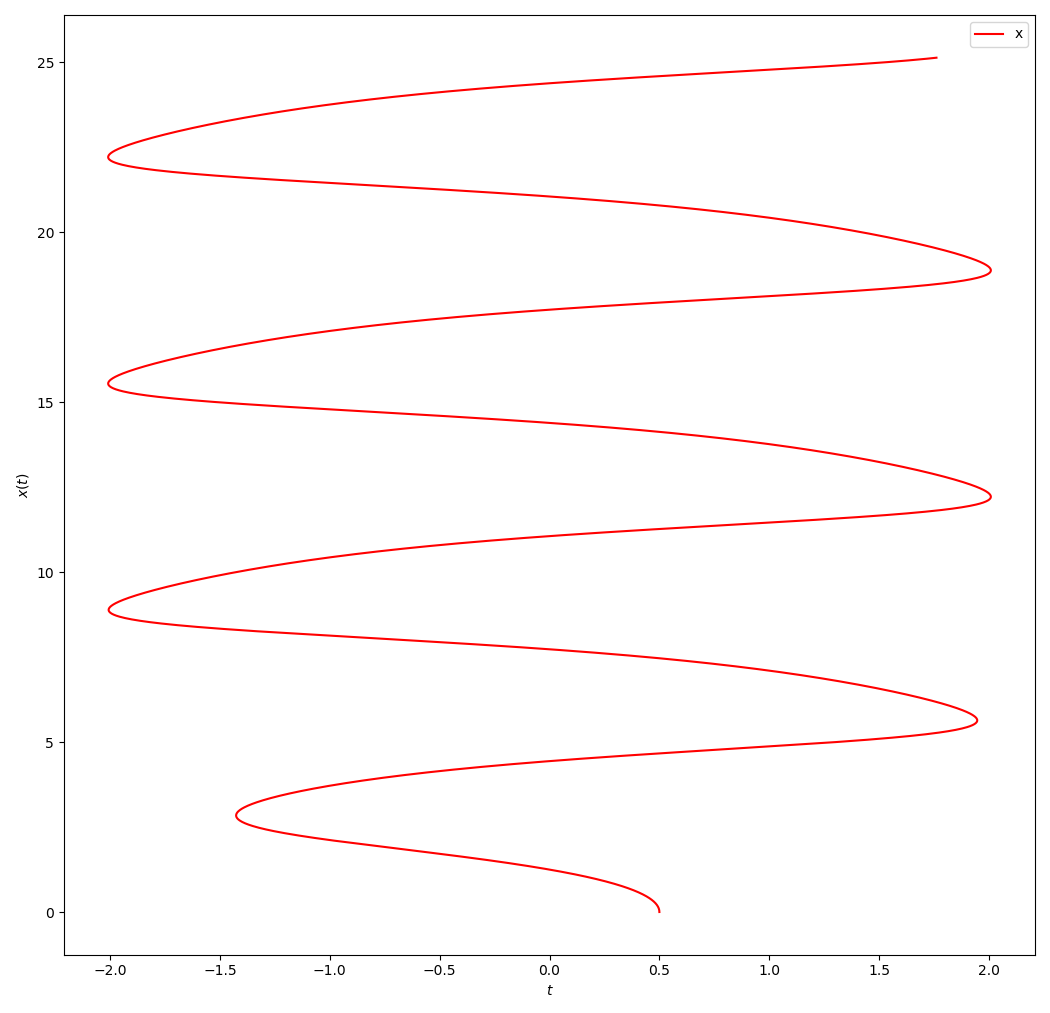
\includegraphics[scale=0.6]{./Cod_74/x(t)_t}
  \end{center}
\end{figure}

\clearpage
\subsubsection*{Q7.4(b) gráfico $\dot x(t)$ vs $t$}

\begin{figure}[!hbt]
  \begin{center}
    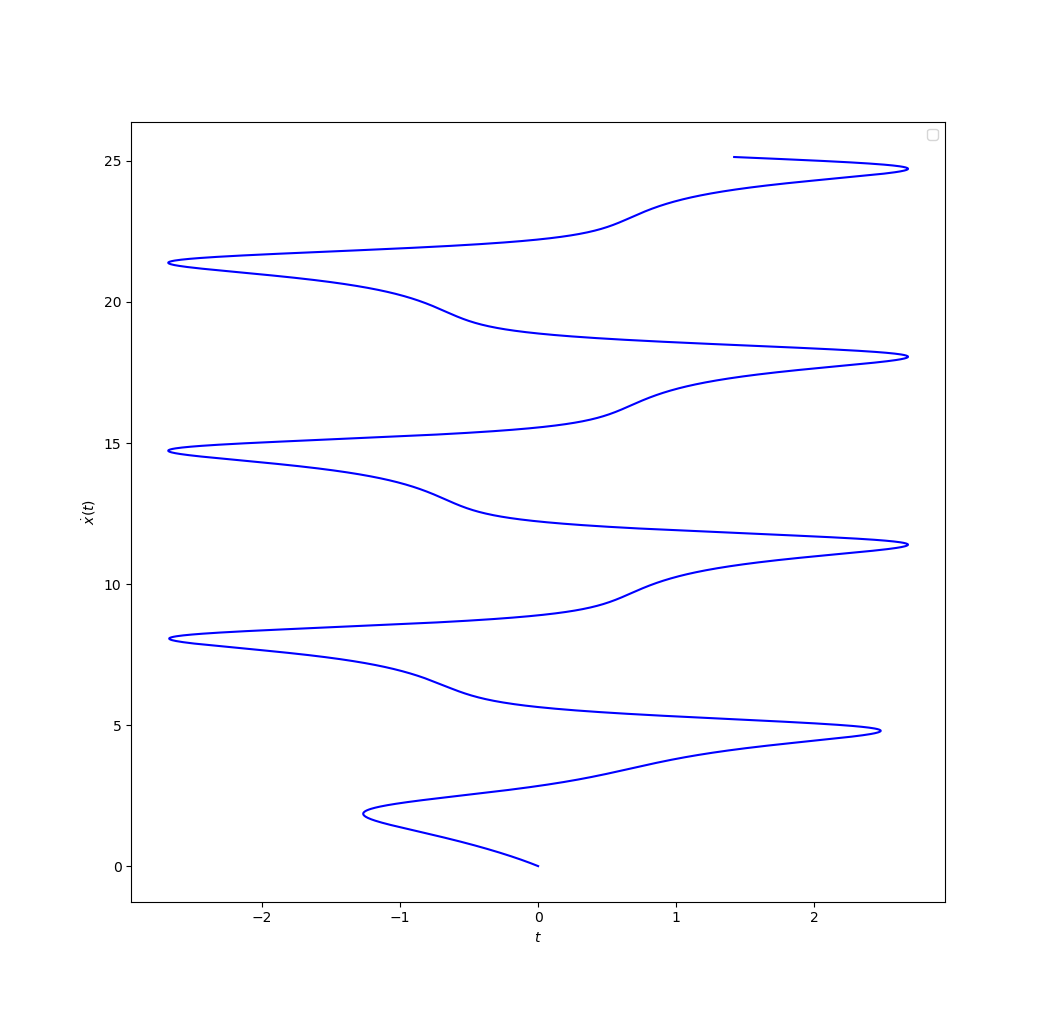
\includegraphics[scale=0.7]{./Cod_74/xdot_t}
  \end{center}
\end{figure}

\clearpage
\subsubsection*{Q7.4(c) gráfico $\dot x(t)$ vs $x$}

\begin{figure}[!hbt]
  \begin{center}
    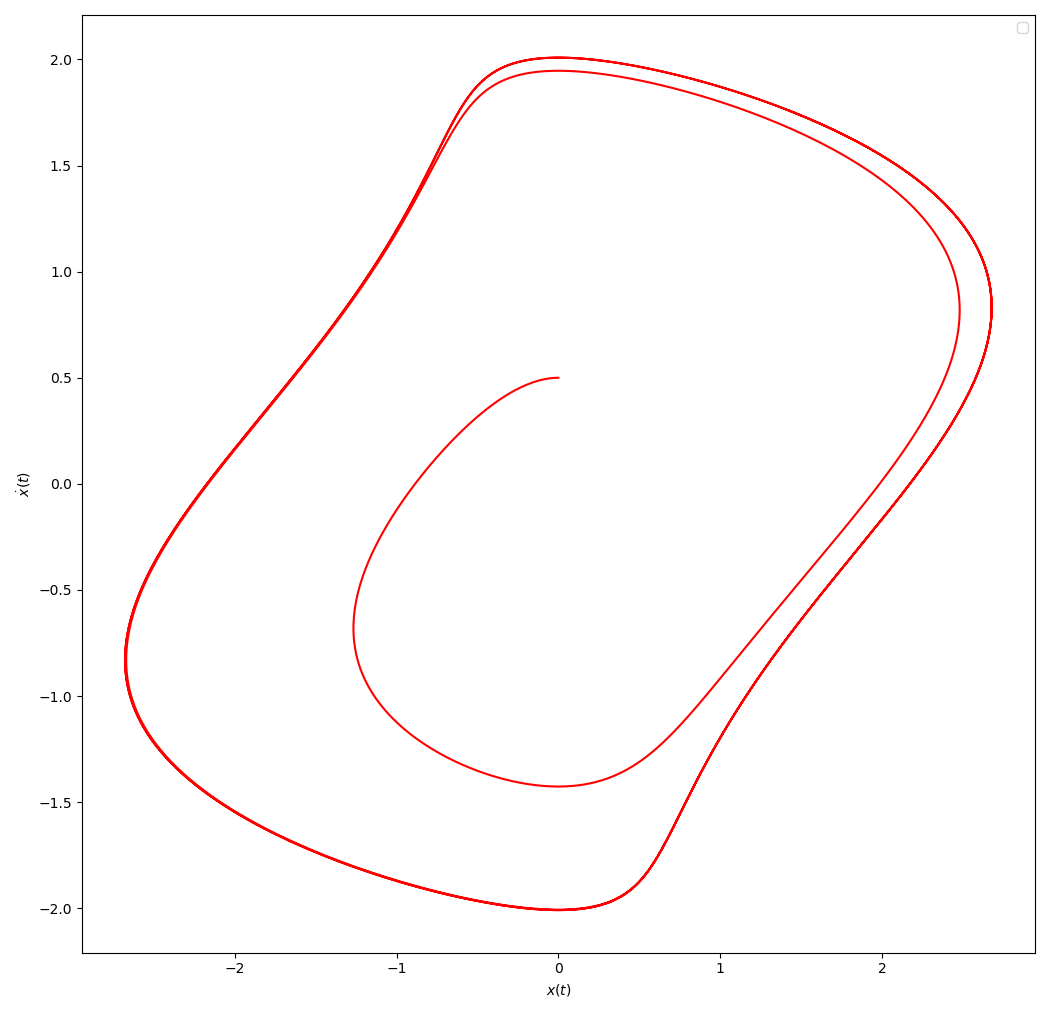
\includegraphics[scale=0.7]{./Cod_74/x(t)_xdot(t)}
  \end{center}
\end{figure}

\clearpage
\section*{Questão 7.5}
\subsubsection*{Q7.5 gráfico $\theta(t)$ vs $\nu(t)$}

\begin{figure}[!hbt]
  \begin{center}
    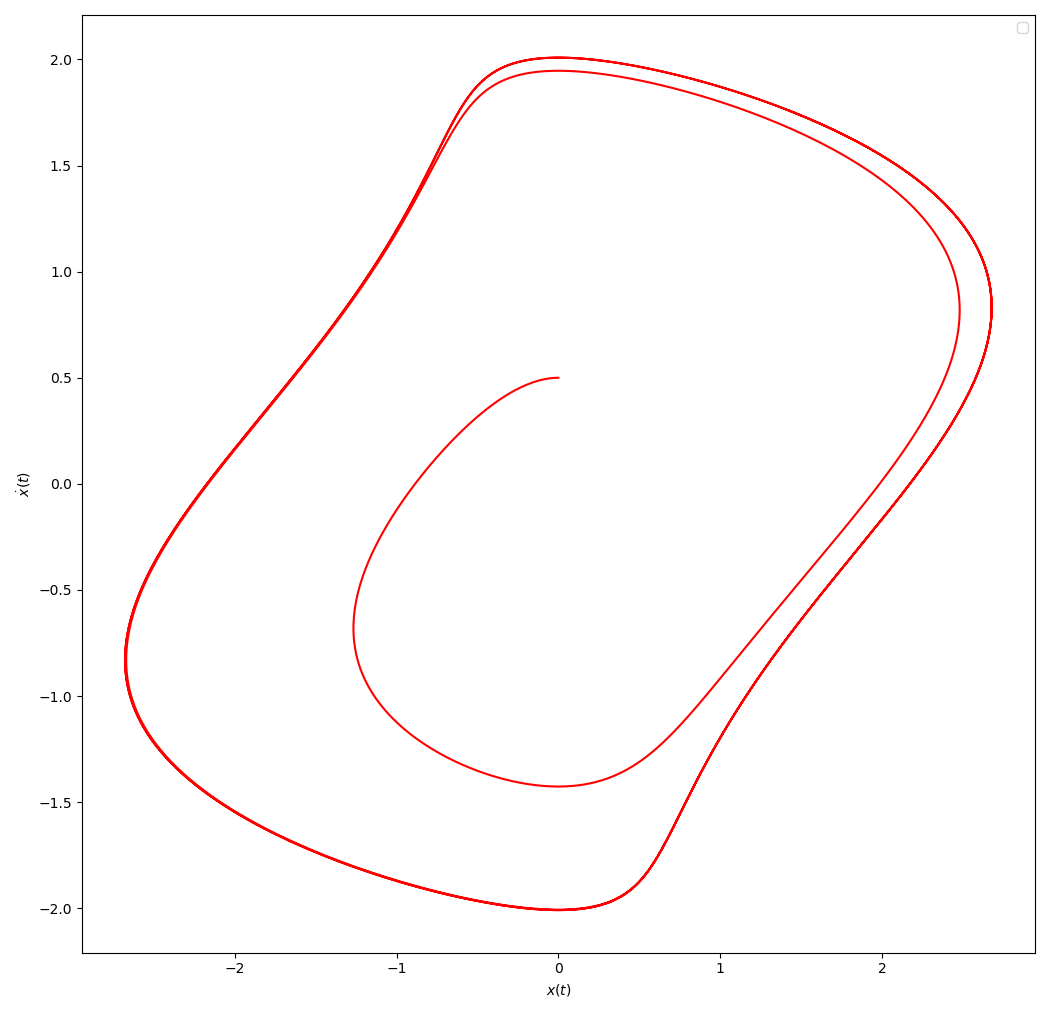
\includegraphics[scale=0.7]{./Cod_74/x(t)_xdot(t)}
  \end{center}
\end{figure}

\end{document}

%%% Local Variables:
%%% mode: latex
%%% TeX-master: t
%%% End:
